\documentclass[a4paper]{article}
\usepackage{hyperxmp}
\usepackage{titling}
\usepackage[colorlinks,linkcolor=blue]{hyperref}
\usepackage{graphicx}
\usepackage{fancyhdr}
\usepackage{a4wide}
\usepackage{xspace}
\usepackage{lastpage}

\newcommand{\myhref}[2]{{\href{#1}{\textcolor{blue}{#2}}}}
\fancyhead[L]{\thetitle}
\fancyhead[R]{\it\thepage\ of \pageref{LastPage}}
\fancyfoot[C]{\centerline{\small \copyright\ \theauthor, 2013. This work is licensed under a \myhref{http://creativecommons.org/licenses/by-sa/3.0/}{Creative Commons Attribution-ShareAlike 3.0 Unported License.}}}
\pagestyle{fancy}

%% PDF meta-data
\hypersetup{%
pdftitle={Assigment 1 for the course on city design. Ideas and Forces That Have Shaped Your City},
pdfauthor={Vitaly Repin},
pdfcopyright={This work is licensed under a Creative Commons Attribution-ShareAlike 3.0 Unported License},
pdfsubject={Designing City},
pdfkeywords={design,city,map},
pdflicenseurl={http://creativecommons.org/licenses/by-sa/3.0/},
pdfcaptionwriter={Vitaly Repin},
pdfcontactcity={Espoo},
pdfcontactcountry={Finland},
pdfcontactemail={vitaly.repin@gmail.com},
pdflang={en}
}

%% City name
\newcommand{\mycity}{Espoo\xspace}
%% Author
\author{Vitaly Repin}
%% Title
\title{Ideas and Forces That Have Shaped My City: \emph{\mycity}}

\date{October, 2013}

\begin{document}
%% Title page

%% Page 1: Map of the city in IXX century
\section{Map of \mycity in IXX century}
%% Change scale size to suit your needs
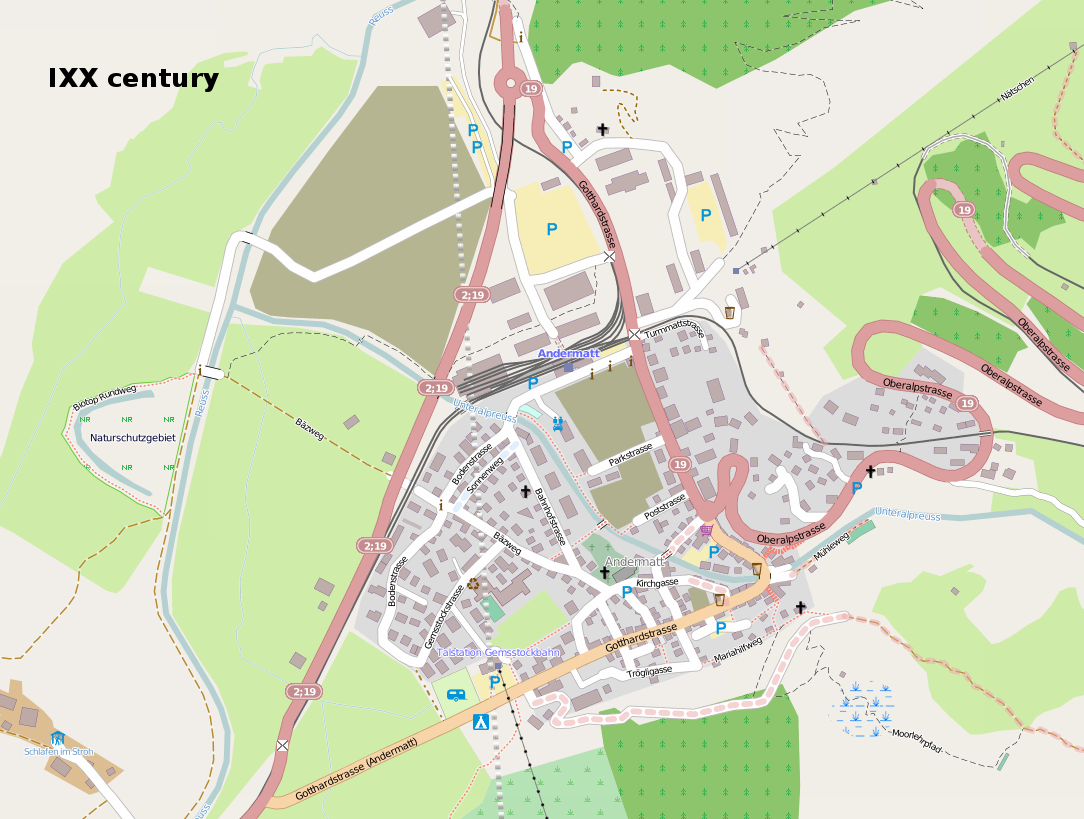
\includegraphics[keepaspectratio,width=\textwidth]{map1}

Comments about the map.

\newpage

%% Page 2: Map of the city in the mid-20th century,
\section{Map of \mycity in the mid-XX century}
%% Change scale size to suit your needs
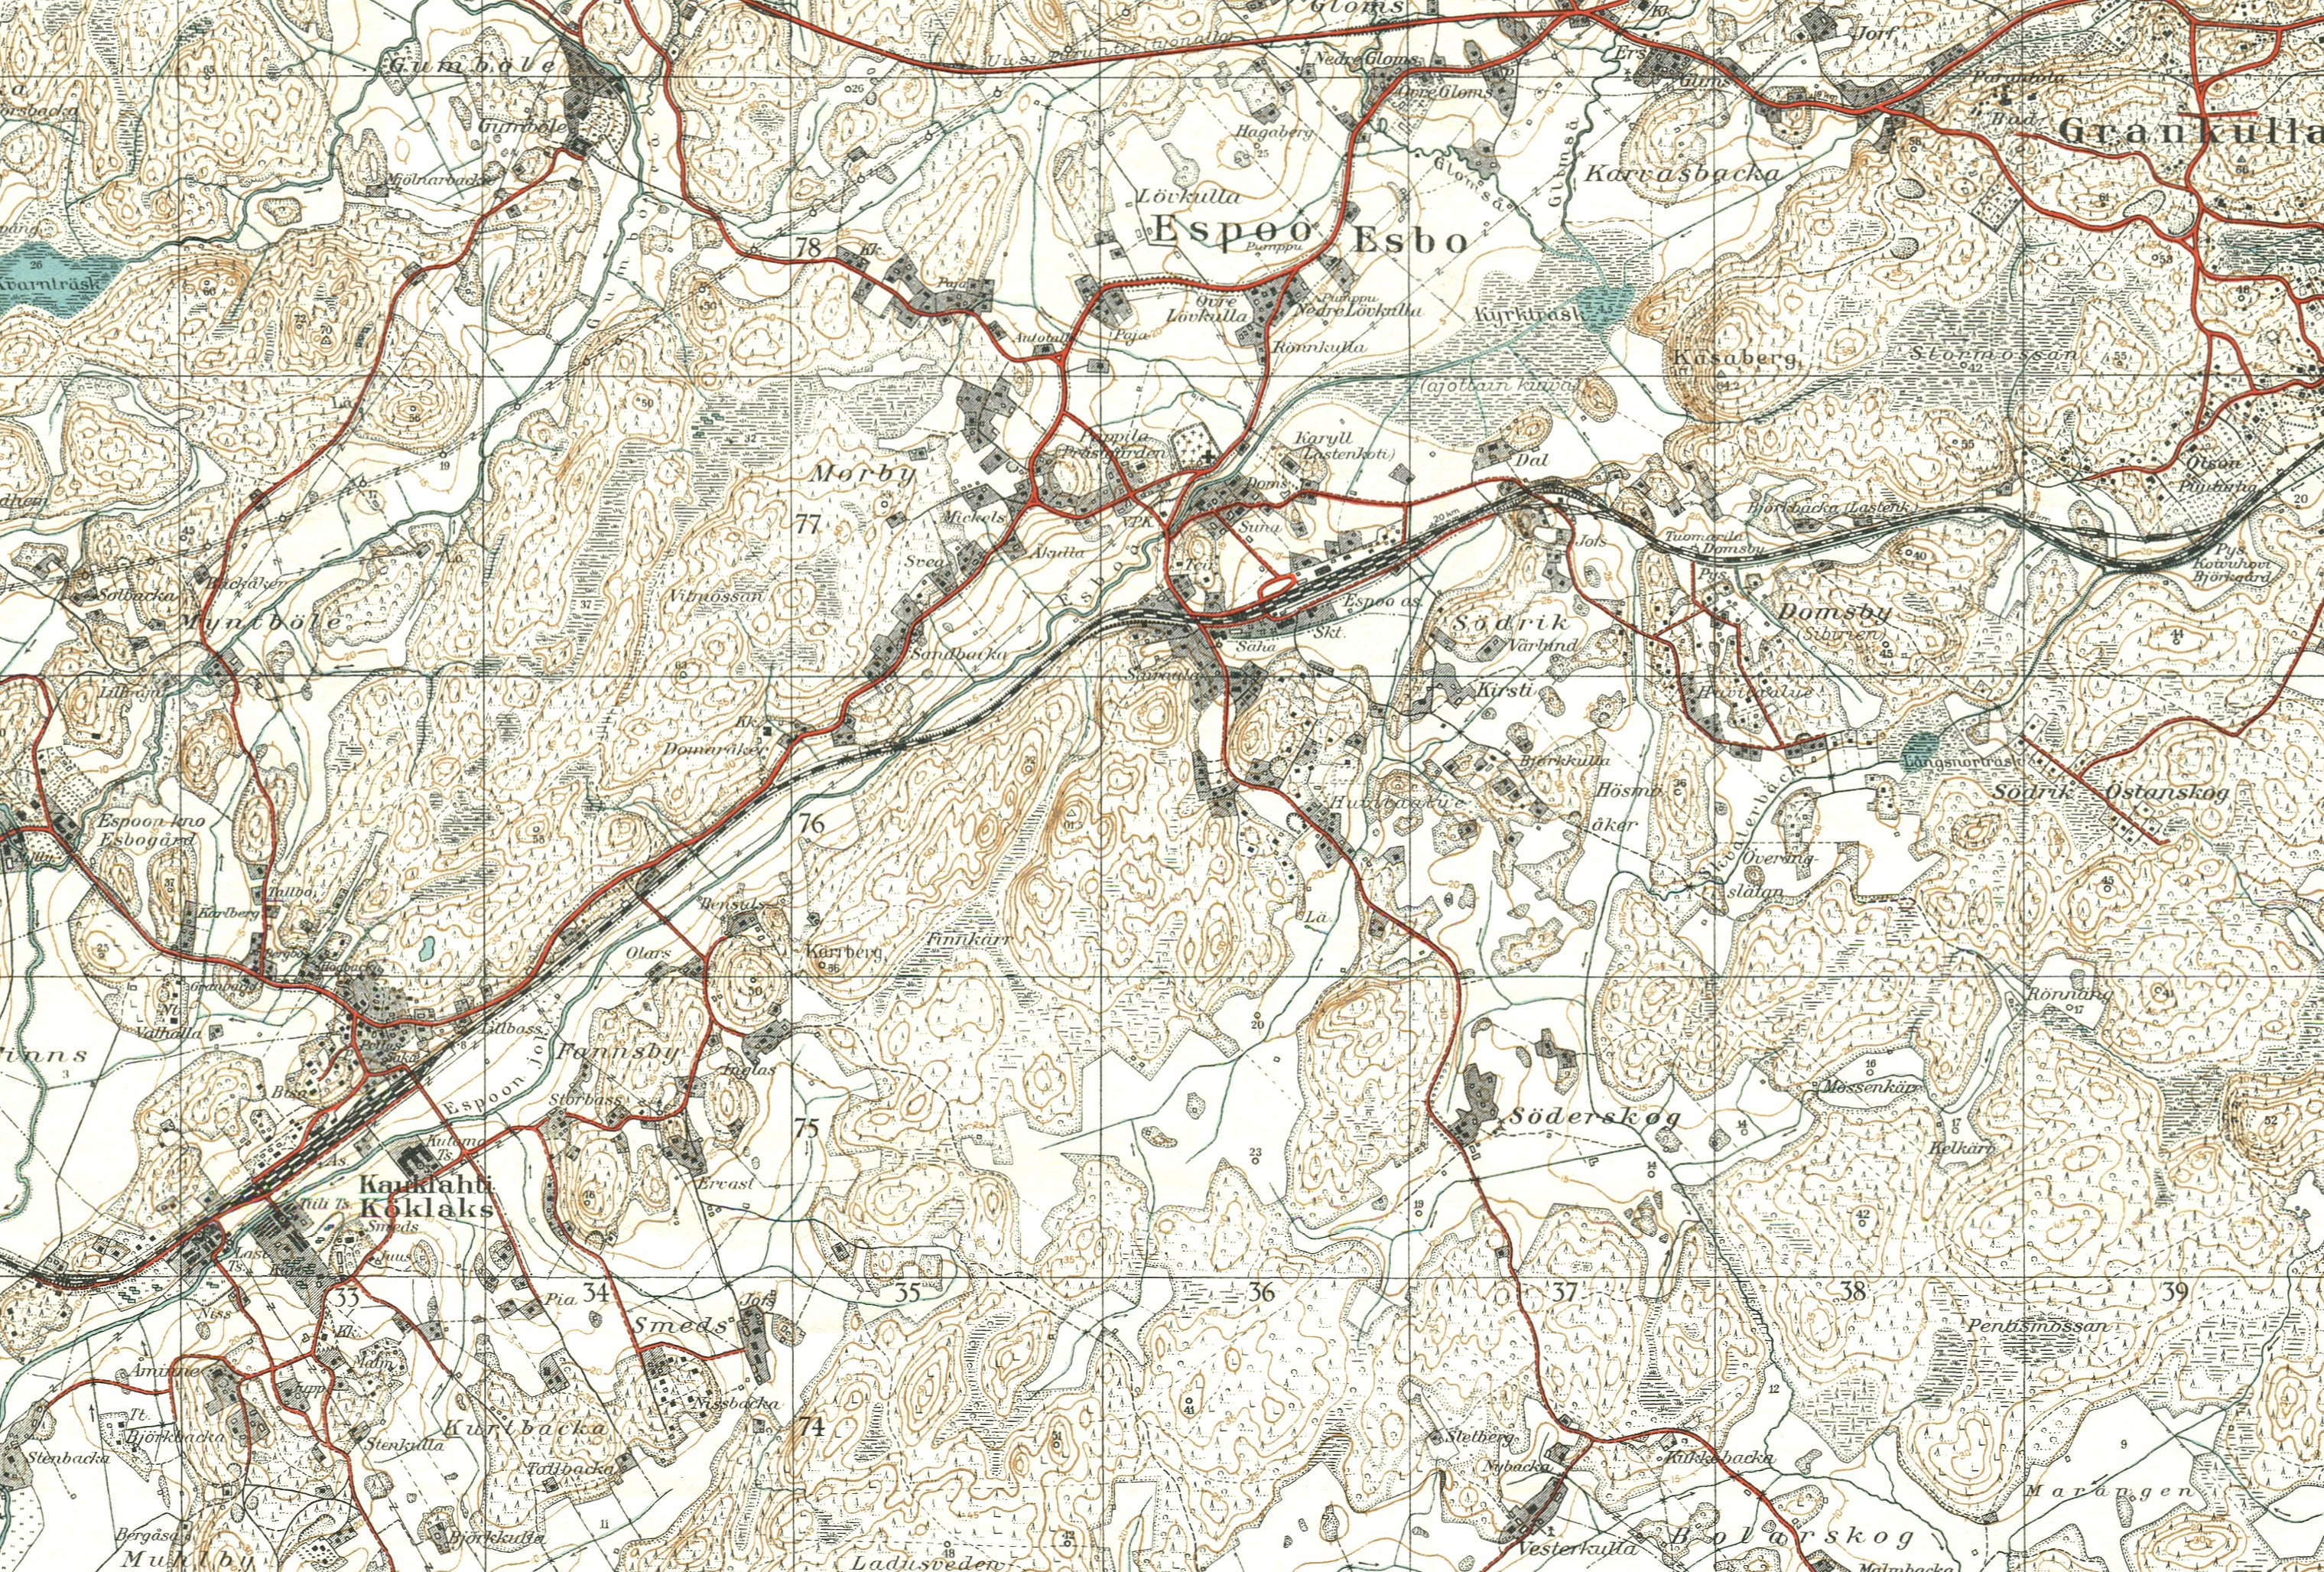
\includegraphics[keepaspectratio,width=\textwidth]{map2}

Comments about the map.

\newpage

%% Page 3: Map of the city today (screenshot from http://www.openstreetmap.org/
\section{Map of \mycity in the year of 2013}
%% Change scale size to suit your needs
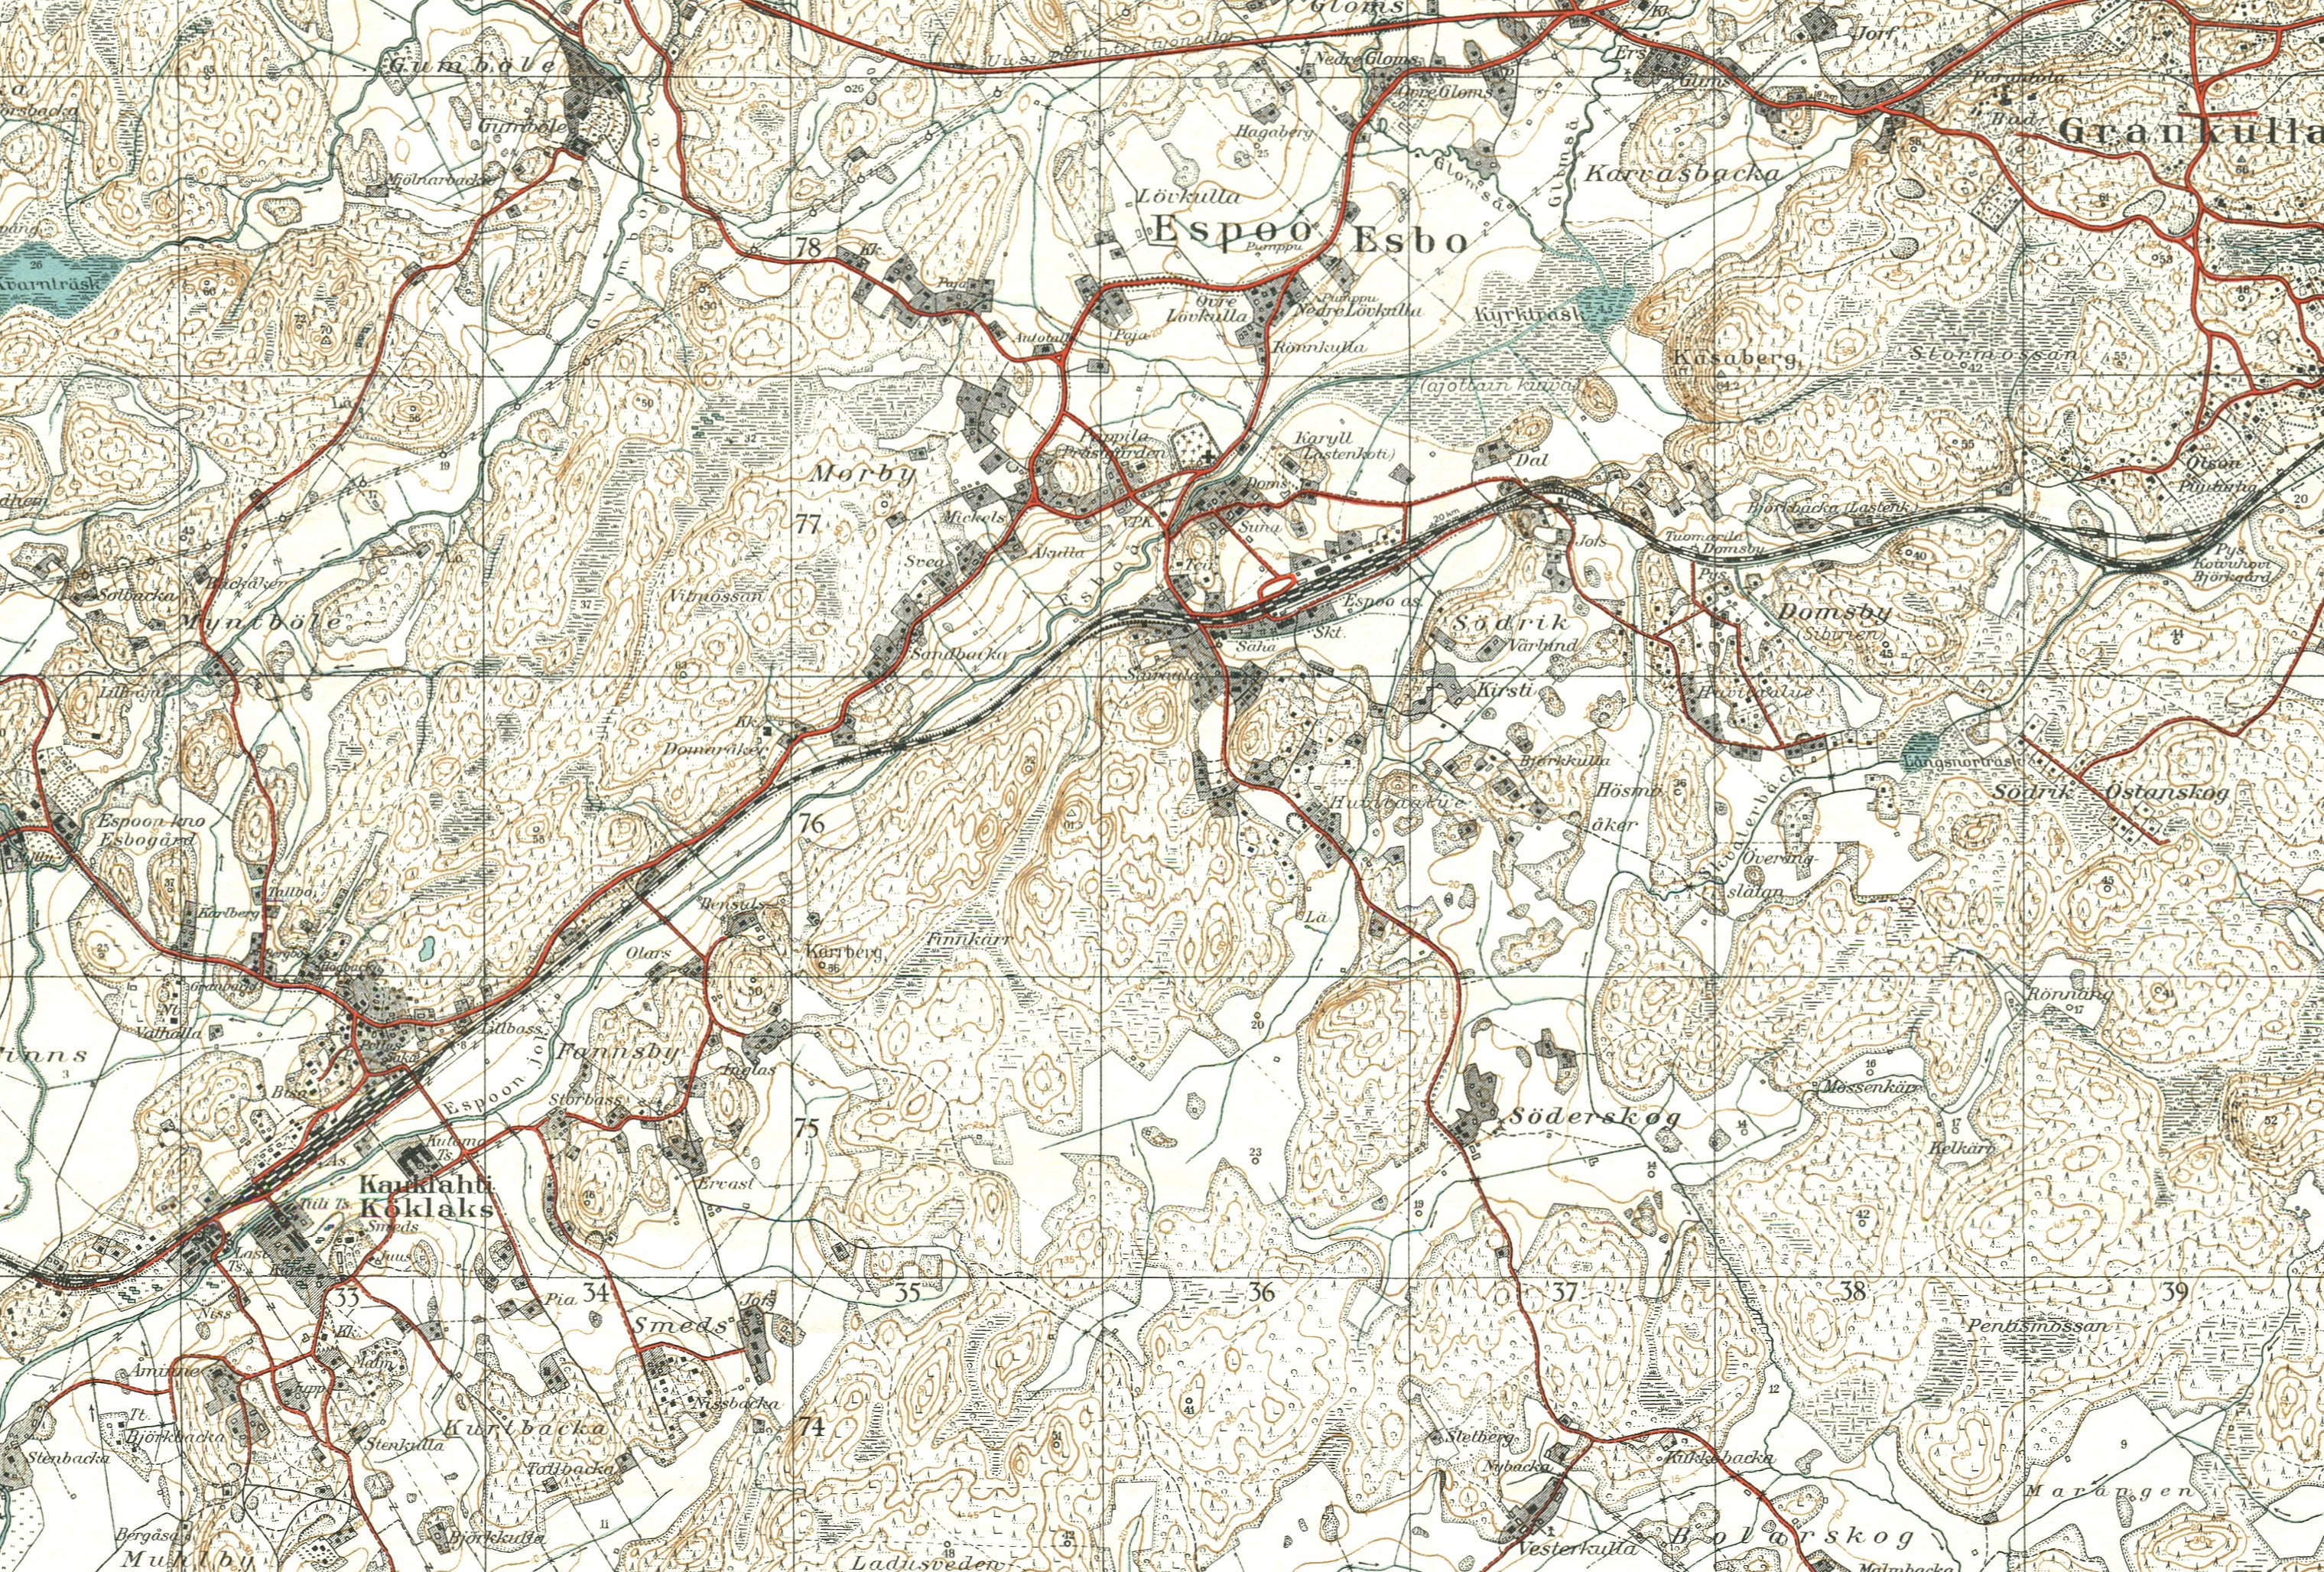
\includegraphics[keepaspectratio,width=\textwidth]{map2}

Comments about the map.

\newpage

%% Page 4: Photographs
\section{Photographs of \mycity}
\begin{tabular}{lp{.4\textwidth}}
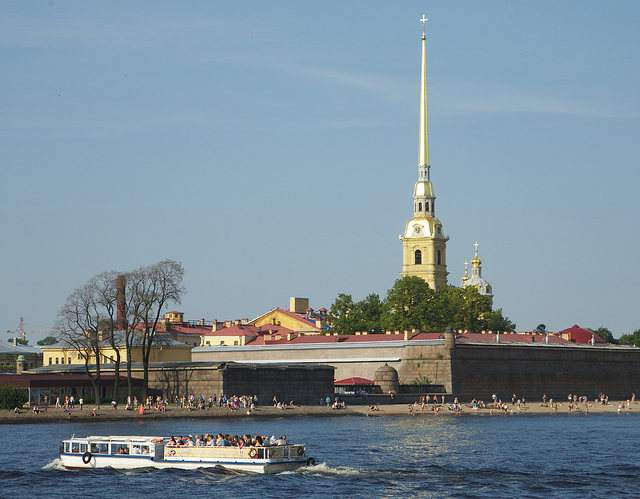
\includegraphics[keepaspectratio,width=.5\textwidth]{photo1} & Comments about photo1\\[.2cm]
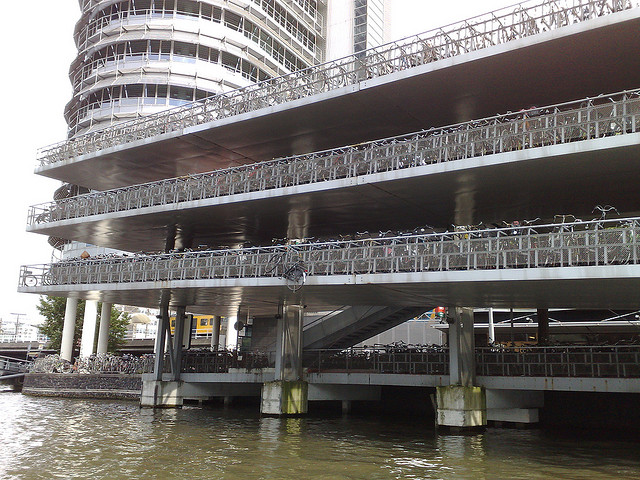
\includegraphics[keepaspectratio,width=.5\textwidth]{photo2} & Comments about photo2\\[.2cm]
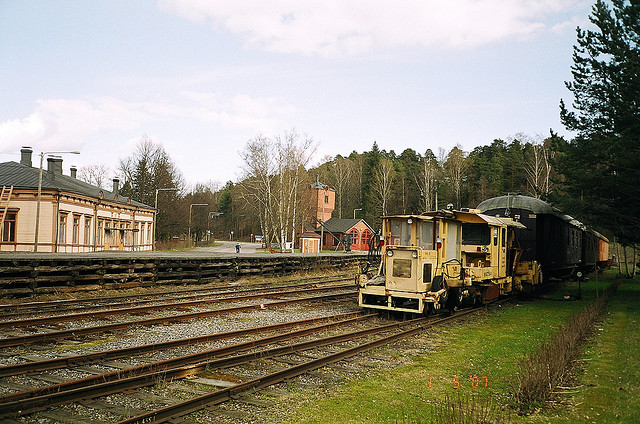
\includegraphics[keepaspectratio,width=.5\textwidth]{photo3} & Comments about photo3\\
\end{tabular}

\end{document}
